\documentclass[
%a4paper, % Use A4 paper size
letterpaper, % Use US letter paper size
]{IEEEtran}
\usepackage[
backend=biber,
style=alphabetic,
sorting=ynt
]{biblatex}
\addbibresource{reference.bib} %Imports bibliography file

\usepackage{graphicx}
\usepackage{subcaption}
\usepackage{multirow}
\usepackage[utf8]{inputenc}
\usepackage[english]{babel}
\usepackage{amsmath}


\author{Jacob Romero}
\title{Project 2: Randomized Optimization}

\begin{document}
	%\lsstyle
	\maketitle
	
	\begin{abstract}
		Random searching has many benefits in real world context as far as solving, or approximately solving notorious computer science problems such as the knapsack or traveling salesman problem. But these randomized searches can be useful in other contexts, especially in cases like optimization which can be directly tied back to machine learning.
	\end{abstract}
	
	\section{Introduction and Problems}
	In this paper we will look at 3 optimization problems, and how they can compare against various optimization algorithms. These algorithms are randomized hill climbing, simulated annealing, genetic algorithms, and finally the MIMIC algorithm. At the heart of each of these algorithms is what is known as a fitness function. A fitness function is a function which can score a specific state for a given problem. In the N-Queens problem, this function would return the number of queens which are attacking other queens. Each of these algorithms approaches the task of optimization in a different way. Some use math as the heart of the algorithm, some rely heavily on biological analogy. These difference lead to different benefits and drawbacks for each of the algorithms. We will explore those points in this paper by analyzing them against 3 problems; Knapsack,  Four-peaks, and One Max.
	
	\subsection{Knapsack}
	The Knapsack optimization problem is a very hard problem in computer science. The goal of this problem is to determine the number of items which maximizes the value carried in the knapsack, while staying at or below the weight capacity for the knapsack. The fitness function is determined by the sum of all the values of the items in the knapsack.
	
	\subsection{Four-Peaks}
	The four peaks problem is different in that rather than have an array of size $N$ and each entry in that array representing a location like the N-Queens problem. Instead this problem focuses on a bit string of arbitrary length $N$, and a threshold $T$. Each entry in string is a one or a zero, and for this problem there are four global maxima (hence the name four peaks). The maxima are a bit string of all 1's, all 0's, or T+1 leading 1's followed by all 0's, or T+1 leading 0's followed by all ones.
	
	\subsection{One-Max}
	For the One-Max problem this is a pretty straightforward problem. In the problem consists of a bit string of 1's and 0's of length $N$. With a fitness function defined as \\ $Fitness(x) = \sum_{i=0}x_i$ 
	
	\section{Algorithms}
	\subsection{Randomized Hill Climbing}
	This algorithm attempts to find maxima of a fitness function by finding the best neighbor or an approximately best neighbor from the current state. This process repeats until there is no improvements that can be made.
	
	\subsection{Simulated Annealing}
	Simulated Annealing is a similar to hill climbing, in that the core of the algorithm attempts to find the best next state to transition to. The twist of this algorithm is the idea of exploration, using a $Temperature (T)$ variable. This acceptance probability of the new state is defined as: \\
	\begin{math}
		P(x,x_t,T) = \begin{cases}
			1 &  \text{if $fitness(x_t) > fitness(x)$} \\
			e \cdot \frac{fitness(x_t) - fitness(x)}{T} & \text{otherwise}
		\end{cases}
	\end{math} \\
	This acceptance probability allows the simulated annealing algorithm to take steps which may be inefficient but in the long run may allow the algorithm to get over the trap of getting stuck in a local optimum, that may not necessarily be the global optimum.
	
	\subsection{Genetic Algorithms}
	While the first two algorithms draw from a natural analogy of hill climbing, and annealing in metallurgy. Genetic algorithms core relies around a strong influence from biology. The idea is that a population of various states are generated. A portion of the top evaluated entries in the population are kept, and breed among other high performing states. The algorithm then also may select at random a new state to mutate in a random way, introducing some exploration into the algorithm. This process repeats for a specified number of iterations, or until there is not more improvement between generations.
	
	\subsection{MIMIC}
	Finally the MIMIC algorithm is the more complicate of the optimization algorithms. This algorithm generates points from a uniform distribution of points, $p^{\theta}(x)$, we then set $\theta = \theta_{t+1} = n^{th}$ percentile. Finally retain only those sample where $fitness(x) \ge \theta_{t+1}$. This algorithm repeats until convergence or max iterations is reached.
	
	\section{Experiments}
	\subsection{Procedure}
	As mentioned the goal of this paper is to explore various aspects of the algorithms listed above. As such we will run each algorithm against the three problems detailed above (N-Queens, Four-Peaks, One-Max), additionally we will see how well the hill climbing, simulated annealing, and genetic algorithms perform in the use of finding the weights for a neural network.
	
	To keep the algorithms on an even ground, between all three of the optimization problems shared parameters will be held constant between algorithms. Additionally parameters for all algorithms will be help constant across problems as well. Each algorithm will use 100 max attempts as improving the fitness score, before quitting early, and a max of 1000 iterations in total. Additionally all algorithms will use the same random seed to avoid variance between runs and experiments. Individual parameters are;
	
	\begin{table}[]
		\begin{tabular}{ll}
			Algorithm            & Parameter                                                                             \\
			Random Hill Climbing & Restarts - 5                                                                          \\
			Simulated Annealing  & Geometric decay schedule                                                              \\
			Genetic Algorithm    & \begin{tabular}[c]{@{}l@{}}Population - 100\\ Mutation Probability - 0.1\end{tabular} \\
			MIMIC                & \begin{tabular}[c]{@{}l@{}}Population - 100\\ Keep percentage - 0.25\end{tabular}    
		\end{tabular}
	\end{table}

	\subsection{Problem 1 - Knapsack}
	\begin{figure}[h]
		\begin{subfigure}{.5\textwidth}
			\centering
			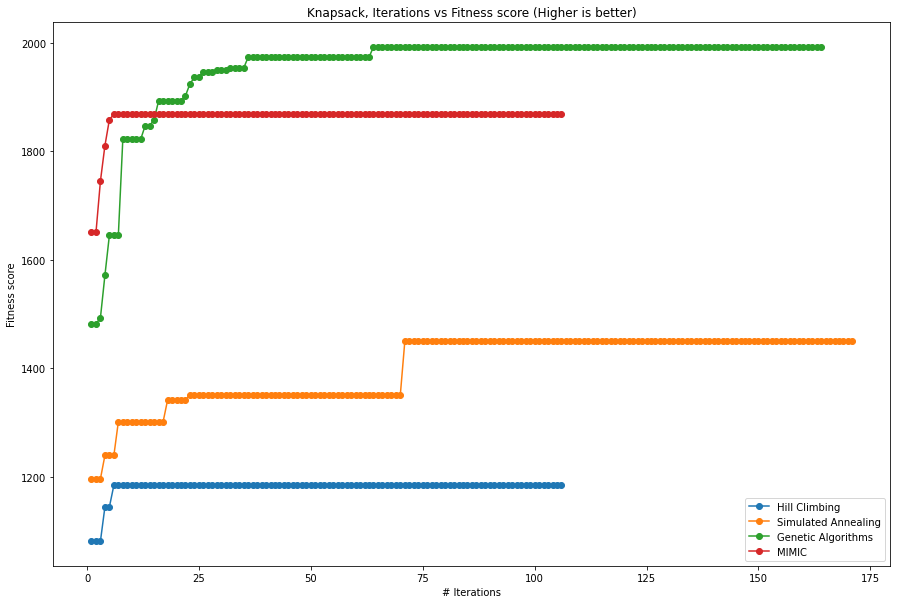
\includegraphics[width=.8\linewidth]{./images/exp1FitnessScore.png}
			\caption{Each algorithm's fitness value vs the number of iterations the algorithm ran.}
			\label{fig:exp1Score}
		\end{subfigure}
		\begin{subfigure}{.5\textwidth}
			\centering
			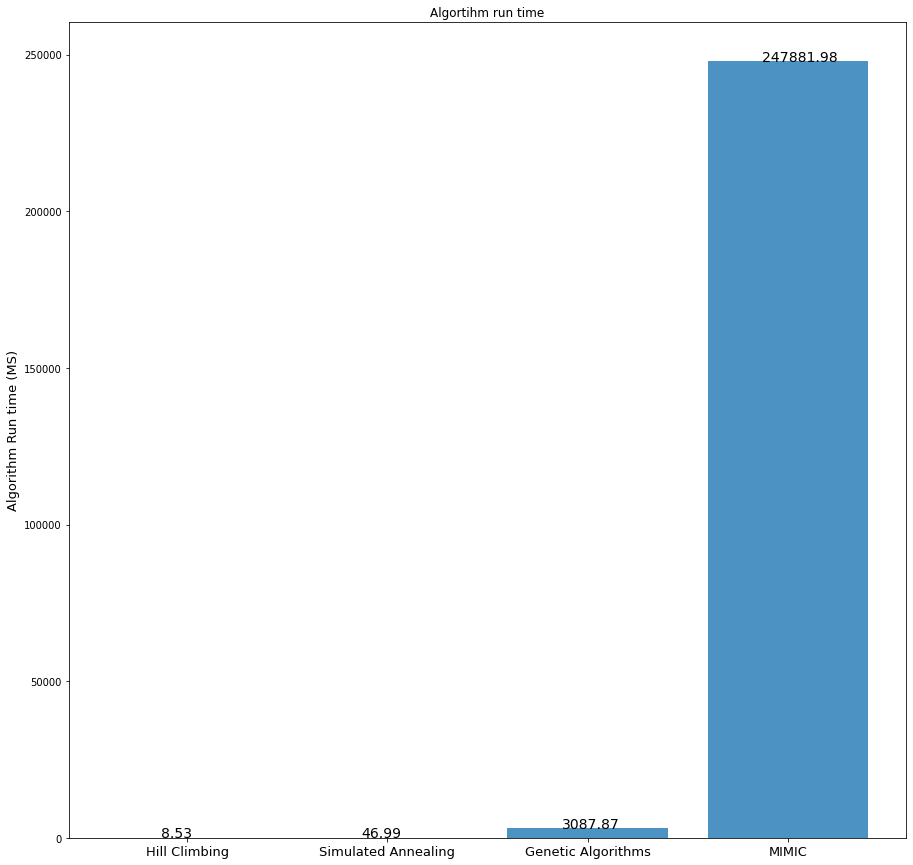
\includegraphics[width=.8\linewidth]{./images/exp1Runtime.png}
			\caption{The time it took for each algorithm to run over the course of its number of iterations.}
			\label{fig:exp1Runtime}
		\end{subfigure}
	\end{figure}

	\begin{center}
		\begin{table}
			\begin{tabular}{ll}
				Algorithm            & Number of iterations until convergence \\
				Random Hill Climbing & 106                                    \\
				Simulated Annealing  & 171                                    \\
				Genetic Algorithm    & 164                                    \\
				MIMIC                & 106                                   
			\end{tabular}
			\caption{Experiment 1 - number of iterations until convergence.}
			\label{table:exp1data}
		\end{table}
	\end{center}

	For the first experiment I ran all the algorithms against the Knapsack problem. For this experiment it gives some interesting results. We can see from Figure \ref{fig:exp1Score} how each of the algorithms behaves in terms of the fitness score vs the number of iterations. For this we can see that genetic algorithms was able to perform very well. This could be due to the way the state space works for this problem because its possible that a mix of the given states may yield a better result. Where as there is a lot of possible states which have low values, or are invalid state (greater than the max weight of the knapsack). Because of this the genetic algorithm is able to take advantage of the mixing of states via the breeding mechanic.
	
	The important thing to note though is that the number of iterations all seem to get stuck fairly early on. We can subtract 100 from the final iteration count from the table \ref{table:exp1data} due to the fact that the algorithms will quit early if not improvement is made after 100 iterations.
	
	Lastly looking at the run times of each algorithm we can see that while genetic algorithms has the highest fitness score. It is random hill climbing and simulated annealing are the better performers in terms of wall clock time. This is important to call out because we will see this trend continue in the later experiments as well. In addition we can see that the iterations of MIMIC were the lowest but the wall clock time was much longer than then genetic algorithm which runs in just 1\% of the time of MIMIC. But each of the following algorithms will show how MIMIC is powerful in reaching a steady state faster than other algorithms.

	\begin{figure}[h]
		\centering
		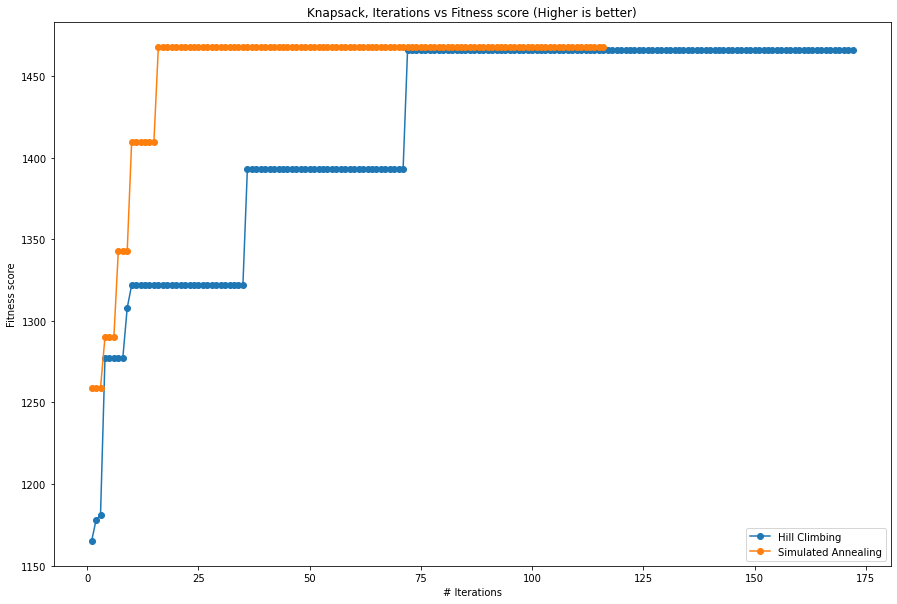
\includegraphics[width=.9\linewidth]{./images/exp1SaVsHc.png}
		\caption{Simulated Annealing with an arithmetic decay schedule vs Hill climbing}
		\label{fig:exp1SaVsHc}
	\end{figure}
	
	\subsubsection{Simulated Annealing behavior}
	One last Interesting note is how simulated annealing behaves. As mentioned in the description of the algorithm, simulated annealing will attempt to perform a type of exploration, by balance its exploitation of the state space search via the temperature parameter, and cooling the temperature according to some decay schedule. We can see how this behavior changes in \ref{fig:exp1SaVsHc}, which changes from a geometric decay schedule, to a more aggressive arithmetic schedule, which subtracts 0.25 from the temperature until a minimum temperature of 0 is reached. In this case we can see that there is much less exploration occurring unlike in the first graph, and the simulated annealing algorithm starts to converge to random hill climbing.
	

	\subsection{Problem 2 - Four Peaks}
	\begin{figure}[h]
		\begin{subfigure}{.5\textwidth}
			\centering
			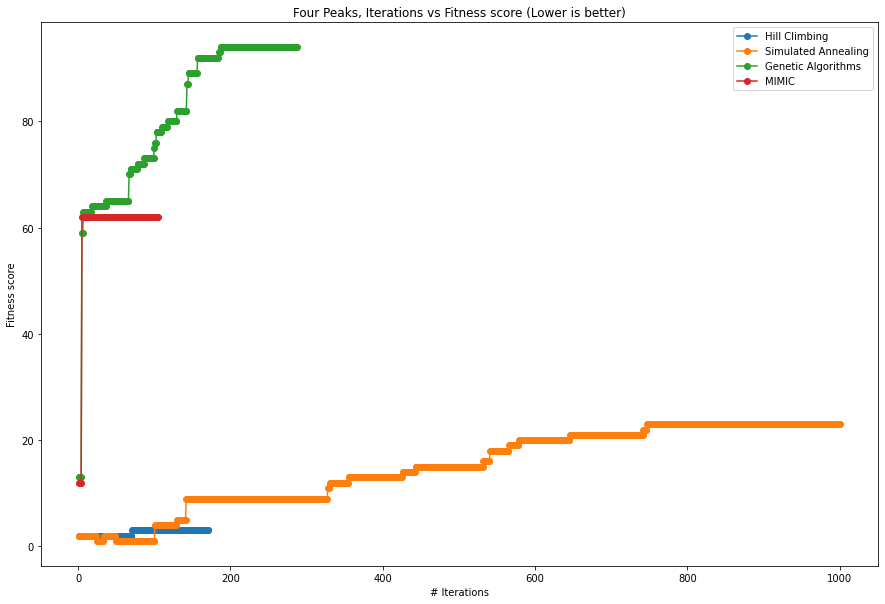
\includegraphics[width=.8\linewidth]{./images/exp2FitnessScore.png}
			\caption{Each algorithm's fitness value vs the number of iterations the algorithm ran.}
			\label{fig:exp2Score}
		\end{subfigure}
		\begin{subfigure}{.5\textwidth}
			\centering
			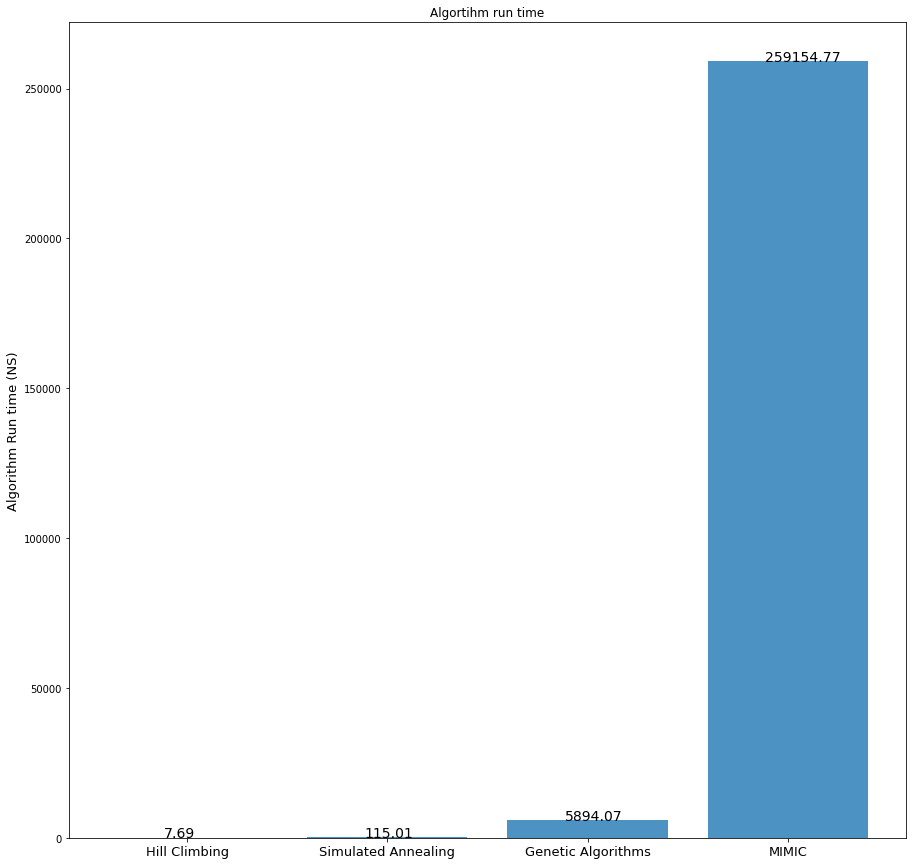
\includegraphics[width=.8\linewidth]{./images/exp2Runtime.png}
			\caption{The time it took for each algorithm to run over the course of its number of iterations.}
			\label{fig:exp2Runtime}
		\end{subfigure}
	\end{figure}

	\begin{center}
		\begin{table}
			\begin{tabular}{ll}
				Algorithm            & Number of iterations until convergence \\
				Random Hill Climbing & 171                                    \\
				Simulated Annealing  & 1000                                    \\
				Genetic Algorithm    & 287                                    \\
				MIMIC                & 105
			\end{tabular}
			\caption{Experiment 2 - number of iterations until convergence.}
			\label{table:exp2data}
		\end{table}
	\end{center}

	Next experiment is running all the algorithms on the four peaks problem. As mentioned in the last section we see a lot of the same trends repeat here. Specifically MIMIC and Genetic Algorithms out performing the other two algorithms, simulated annealing and random hill climbing. While MIMIC did have a much lower number of iterations, it was unable to find a better next state in time to prevent it from stopping early. In this case Genetic algorithm was still able to beat the score found by MIMIC. In addition to finding a higher valued state. Genetic algorithm was also much faster, taking only about 2\% of the time as MIMIC. Again the genetic algorithm performs well due to the fact that the fitness function works by the checking if the array is mostly 0's followed by 1's, mostly 1's followed by 0's, all 1's or all 0's. Again the breeding aspect of genetic algorithms may play an important role here.
	
	\subsection{Problem 3 - One Max}
	\begin{figure}[h]
		\begin{subfigure}{.5\textwidth}
			\centering
			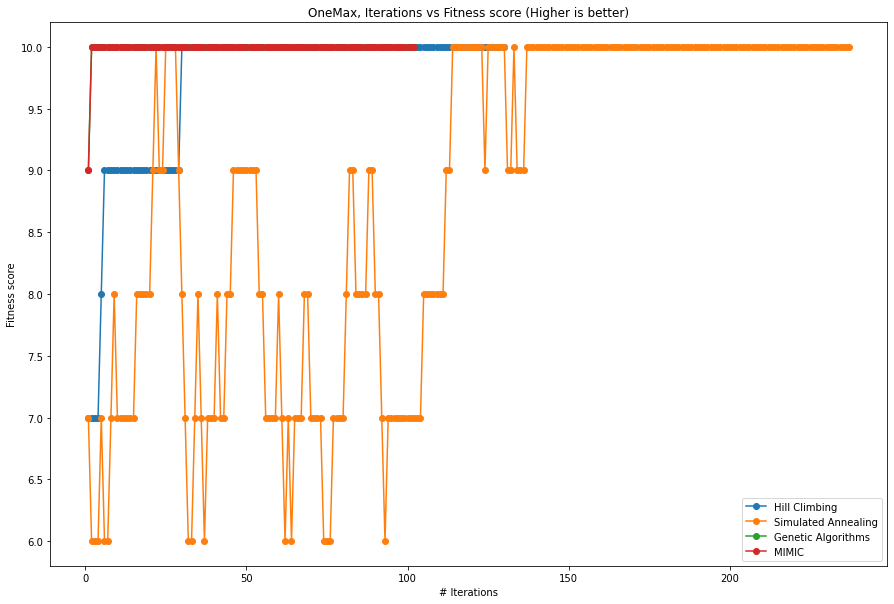
\includegraphics[width=.8\linewidth]{./images/exp3FitnessScore.png}
			\caption{Each algorithm's fitness value vs the number of iterations the algorithm ran.}
			\label{fig:exp3Score}
		\end{subfigure}
		\begin{subfigure}{.5\textwidth}
			\centering
			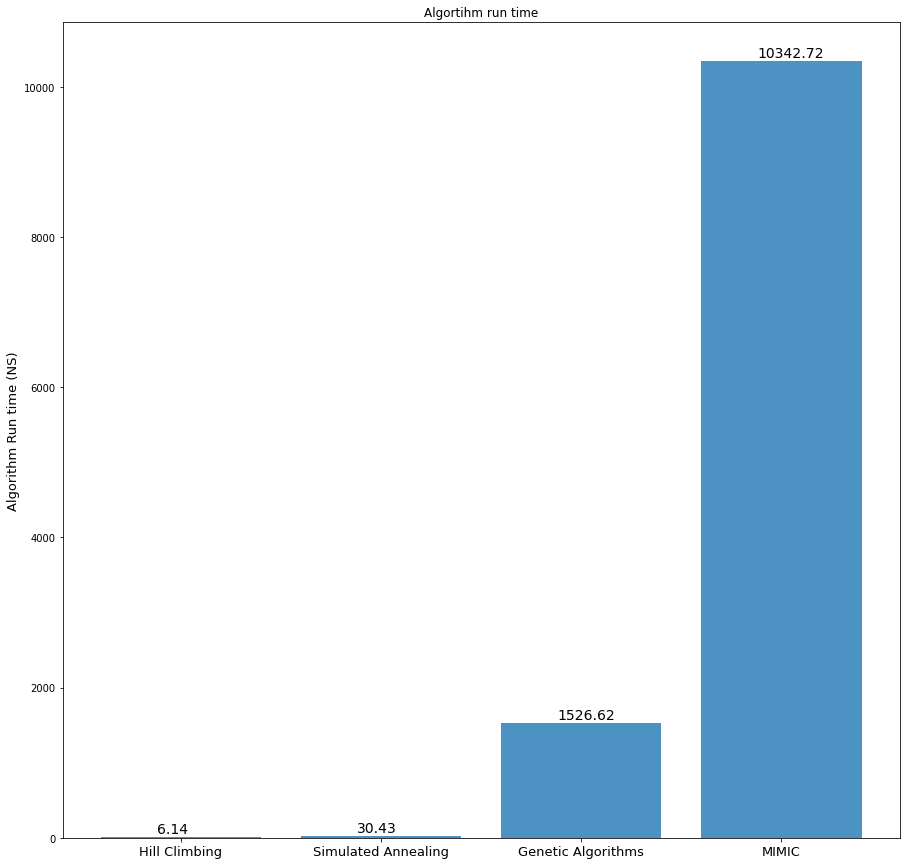
\includegraphics[width=.8\linewidth]{./images/exp3Runtime.png}
			\caption{The time it took for each algorithm to run over the course of its number of iterations.}
			\label{fig:exp3Runtime}
		\end{subfigure}
	\end{figure}

	\begin{center}
		\begin{table}
			\begin{tabular}{ll}
				Algorithm            & Number of iterations until convergence \\
				Random Hill Climbing & 130                                    \\
				Simulated Annealing  & 237                                    \\
				Genetic Algorithm    & 102                                   \\
				MIMIC                & 102                                  
			\end{tabular}
			\caption{Experiment 3 - number of iterations until convergence.}
			\label{table:exp3data}
		\end{table}
	\end{center}

	For the final of our simple optimization problems the One Max problem is very straight forward. Where the fitness is simply determined by the number of 1's in the state vector. Because of the simplicity of this algorithm we can see from figure \ref{fig:exp3Runtime} that all the algorithms where able to find the global optimum of 10 (the length of the state vector $X$). Because of this again we look at iterations, where again as MIMIC/Genetic Algorithm both were able to converge fast. However for this case due to the simplicity of the fitness function, when looking at the wall clock times of random hill climbing, and simulated annealing, they are vastly superior to the other two algorithms, MIMIC and genetic algorithms.

	\subsection{Problem 4 - Neural Network weight optimization}
	\begin{figure}[h]
		\begin{subfigure}{.5\textwidth}
			\centering
			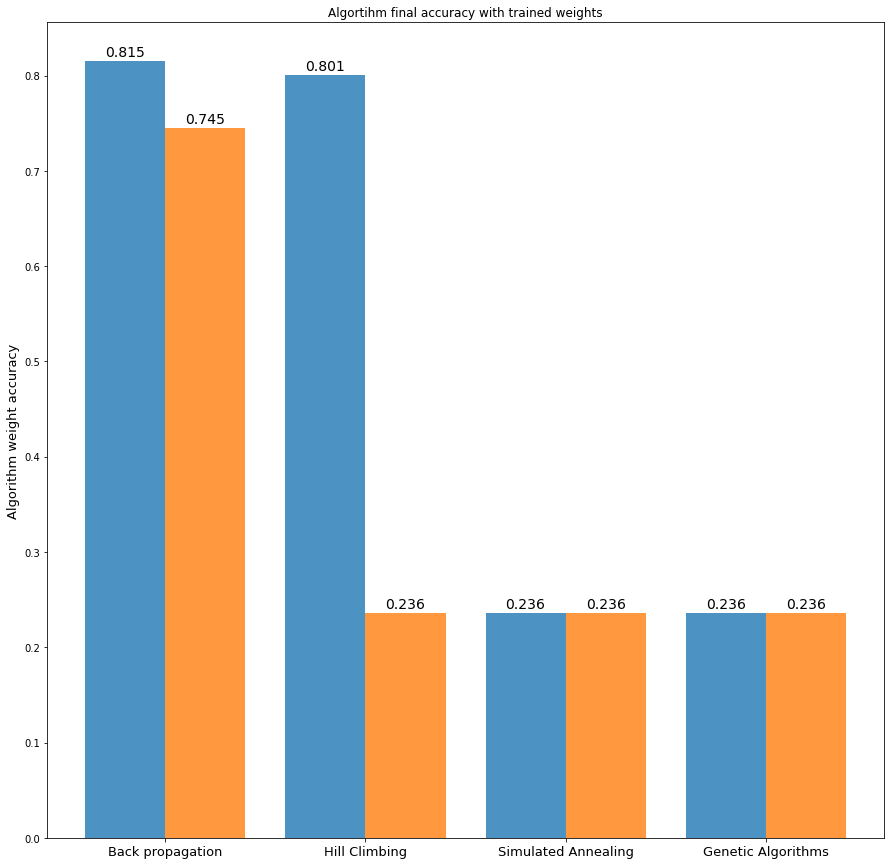
\includegraphics[width=.8\linewidth]{./images/nnTrainAcc.png}
			\caption{Neural network training accuracy by optimization algorithm.}
			\label{fig:exp4Score}
		\end{subfigure}
		\begin{subfigure}{.5\textwidth}
			\centering
			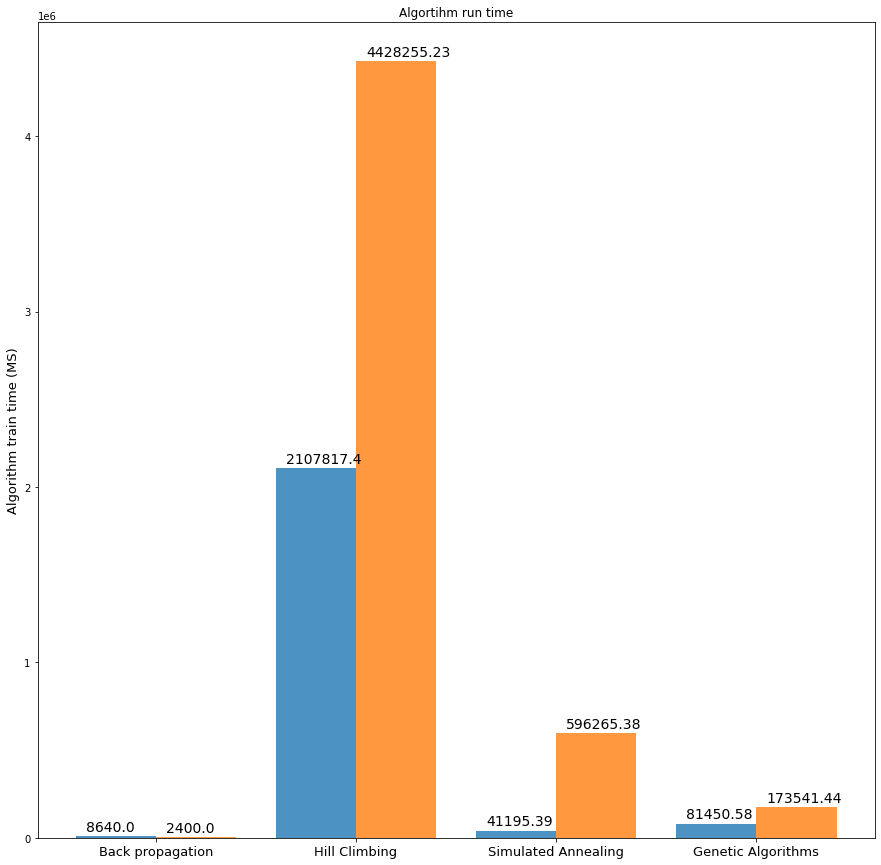
\includegraphics[width=.8\linewidth]{./images/nnTrainTime.png}
			\caption{Neural network training times by optimization algorithm..}
			\label{fig:exp4Runtime}
		\end{subfigure}
	\end{figure}
	
	For our last experiment we want to tie in the optimization algorithms directly with machine learning. With many machine learning algorithms we are trying to optimize some function to reduce an error in our data prediction. With that we can then transfer our algorithms directly to a case such as training weights for a neural network. Using the two datasets from Project 1, dataset 1 being the income classification of citizens from the U.S. census. While the second dataset is the default status for customers of a Taiwanese bank.
	
	This is very interesting on the second dataset, is the fact that the all algorithms preformed the same as far as accuracy on the testing set goes. This implies that because of the complication of the state space, as the size of the neural network was set to $1 \times 100$ network (1 layer, 100 nodes). Where as the first dataset was able to achieve higher (almost) close to the back propagation score. This neural network was much simpler at $1 \times 10$. It is also worth noting that as we increase the size of the neural network the number of possible next states that can be generate goes up which explains also why the training accuracy is not able to be improved as well as back propagation.
	
	On the training time side, it is worth noting that all algorithms performed worse than standard back propagation, by a large margin. This could be attributed to the fact that randomized optimization algorithms do not have as much sophistication as the back propagation algorithm. Which takes derivative with respect to each of the individual weight, and adjusts them accordingly. This reduces the state space that is explored unlike the optimization algorithms which explore with no domain knowledge of the neural network.
	
	\section{Conclusion}
	We have looked at the power of optimization algorithms, including randomized hill climbing, simulated annealing, genetic algorithms, and MIMIC. Each of these algorithms draws some inspiration from nature. Each of the approaches of these algorithms has benefits and drawbacks that we explored in this paper. From the type of fitness functions, and state spaces that genetic algorithms performs well in. The algorithm wall clock times for each and how MIMIC while fast in terms of the number of iterations, takes the longest to run in our experiment problems. Finally we looked at how these optimization algorithms can be used to get a set of weights for a neural network which can possible get close to the accuracy of back propagation.
	
	\nocite{*}
	\printbibliography[
	heading=bibintoc,
	title={References}
	] %Prints the entire bibliography with the title "Whole bibliography"
\end{document}\textsl{}